\chapter{Funciones}

\section{Las funciones y sus gráficas}

    %--------------------definición 1.1.
    \begin{tcolorbox}[colframe=white]
	\begin{def.}
	    Una función $f$ de un conjunto $D$ a un conjunto $Y$ es una regla que asigna a cada elemento $x \in D$ un solo o único elemento $f(x) \in Y$\\
	\end{def.}
    \end{tcolorbox}

    %--------------------definición 1.2.
    \begin{tcolorbox}[colframe=white]
	\begin{def.}
	    Cuando definimos una función $y = f(x)$ mediante una fórmula, y el dominio no se establece de forma explícita o se restringe por el contexto, se supondrá que el dominio será el mayor conjunto de números reales $x$ para los cuales la fórmula proporciona valores reales para $y$ , el llamado \textbf{dominio natural}.\\\\
	    Cuando el rango de una función es un subconjunto de números reales, se dice que la función tiene \textbf{valores reales (o que es real valuada)}\\
	\end{def.}
    \end{tcolorbox}

    %--------------------definición 1.3.
    \begin{tcolorbox}[colframe=white]
	\begin{def.}[Valor absoluto]
	    $f(x)=\left\{\begin{array}{rcl}
		x&si&x\geq 0\\
		\\ -x&si&x<0\\
	    \end{array} \right.$
	\end{def.}
    \end{tcolorbox}

    %--------------------definición 1.4.
    \begin{tcolorbox}[colframe=white]
	\begin{def.}
	    Sea una funcion definida en un intervalo $I$ y sean $x_1$ y $x_2$ cualesquiera dos puntos en $I$ 
	    \begin{enumerate}[\bfseries 1.]
		\item Si $f(x_2) > f(x_1)$, siempre que $x_1<x_2$ entonces se dice que $f$ es \textbf{creciente} en $I$.
		\item Si $f(x_2) < f(x_1)$, siempre que $x_1<x_2$ entonces se dice que $f$ es $\textbf{decreciente}$ en $I$.\\
	    \end{enumerate}
	\end{def.}
    \end{tcolorbox}

    %--------------------definición 1.5.
    \begin{tcolorbox}[colframe=white]
	\begin{def.}
	Una función $y=f(x)$ es una 
	    \begin{enumerate}[\bfseries 1.]
		\item Función par de $x$ si $f(-x)=f(x)$.
		\item Función impar de $x$ si $f(-x)=-f(x)$.
	    \end{enumerate}
	Para toda $x$ en el dominio de la función.\\\\
	(Los nombres par e impar provienen de las potencias de $x$).\\
	\end{def.}
    \end{tcolorbox}

    %--------------------definición 1.6.
    \begin{tcolorbox}[colframe=white]
	\begin{def.}
	    Dos variables $x$ e $y$ son \textbf{proporcionales} (una con respecto a la otra) si una siempre es un múltiplo constante de la otra; esto es, si $y=kx$ para alguna constante $k$ distinta de $0$.\\\\
	    Si la variable $y$ es proporcional al recíproco $1/x$, entonces algunas veces se dice que $y$ es \textbf{inversamente proporcional} a $x$ (puesto que $1/x$ es el inverso multiplicativo de $x$).\\

	\end{def.}
    \end{tcolorbox}


\setcounter{section}{0}
\section{Ejercicios}

\begin{enumerate}[\Large \bfseries 1.]

    %--------------------1.
    \item $f(x)=1+x^2$ \\\\
	Respuesta.-\; Al evaluar $1+x^2$ vemos que $x$ se cumple para todos los reales, por lo tanto $f_D=\lbrace x /; \forall \; x \in \mathbb{R} \rbrace$. Luego el rango viene dado por $f_R=\lbrace y=f(x) / y \geq 1 \rbrace$\\\\

    %--------------------2.
    \item $f(x)=1-\sqrt{x}$\\\\
       Respuesta.-\; El dominio viene dado por $f_D=\lbrace x / x \geq 0 \rbrace$. Y el rango viene dado por $f_R = \lbrace y = f(x) / y \leq 1 \rbrace$.\\\\

    %--------------------3.
    \item $F(x)=\sqrt{5x + 10}$\\\\
	Respuesta.-\; Sea $5x + 10 \geq 0$ ya que una raíz par no puede ser no negativo, entonces $x \geq 2$, por lo tanto el dominio viene dado por $f_D=\lbrace x / x \geq -2 \rbrace$. Luego el rango viene dado por $f_R = \lbrace y=f(x) / y \geq 0 \rbrace$.\\\\

    %--------------------4.
    \item $g(x)=\sqrt{x^2 - 3x}$\\\\
	Respuesta.-\; De igual forma al anterior ejercicio, evaluaremos $x^2 - 3x \geq 0$, de donde $x(x-3)\geq 0$, por lo tanto el dominio es $f_D=\lbrace x/\leq x \leq 0 \cup x \geq 3 \rbrace$. Luego el rango viene definido por $f_R=\lbrace y=f(x) / y \geq 0 \rbrace$.\\\\

    %--------------------5.
    \item $f(t)=\dfrac{4}{3-t}$ \\\\
	Respuesta.-\; Sabemos que no se puede dividir un número por $0$. Por lo tanto para hallar el dominio de la función debemos evaluar $3-t=0$, de donde $t=3$, así $f_D=\lbrace t / t\neq 3\rbrace$. Luego el rango viene dado por $f_R=\lbrace y=f(x) / y\neq 0\rbrace$.\\\\

    %--------------------6.
    \item $G(t)=\dfrac{2}{t^2 - 16}$ \\\\
	Respuesta.-\; De igual forma al anterior ejercicio evaluamos $t^2 - 16 = 0$, de donde $(t - 4)(t + 4)=0$, por lo tanto el dominio de la función viene dado por $f_D=\lbrace t / t \neq 4 \land t \neq -4 \rbrace$. Luego el rango viene dado por $f_R=\lbrace y=f(x) / 0 < y \leq - \dfrac{1}{8} \rbrace$ ya que al despejar $x$ nos queda  $x=\sqrt{\dfrac{2}{y} + 16}$ de donde se debe evaluar por un lado $\dfrac{2}{y}$ y por otro $\dfrac{2}{y} - 16 \geq 0$.\\\\

    En los ejercicios $7$ y $8$ ¿Cuál de las gráficas representa la gráfica de una función de $x$? ¿Cuáles no representan a funciones de $x$? Dé razones que apoyen sus respuestas.\\\\

    %--------------------7.
    \item El inciso $a.$ no es una función ya que no cumple con la prueba de la recta vertical ya una función sólo puede tener un valor $f(x)$ para cada $x$ en su dominio. Y el inciso $b.$ no representa la gráfica de una función.\\\\

    %--------------------8.
    \item Los incisos $a.$ y $b.$ no representan a funciones de $x$. El único que no representa una gráfica de una función es el inciso $b.$\\\\

    Determinación de fórmulas para funciones.\\\\

    %--------------------9.
    \item Exprese el área y el perímetro de un triángulo equilátero como una función del lado $x$ del triángulo.\\\\
	Respuesta.-\; El área se representa por $f(x)=\dfrac{\sqrt{3}a^2}{4}$ y el perímetro por $f(x)=3x$\\\\

    %--------------------10.
    \item Exprese la longitud del lado de un cuadrado como una función de la longitud $d$ de la diagonal del cuadrado. Exprese el área como una función de la longitud de la diagonal.\\\\
	Respuesta.-\; La longitud del lado de un cuadrado como función de longitud esta dado por $d=\sqrt{2a^2}$. El área es expresado por $A=\dfrac{d^2}{2}$\\\\

    %--------------------11.
    \item Exprese la longitud del lado de um cubo como una función de la longitud de la diagonal $d$ del cubo. Exprese el área de la superficie y el volumen del cubo como una función de la longitud de la diagonal.\\\\
	Respuesta-.\; La expresión de la longitud del lado del cubo como función de la longitud de la diagonal $d$ del cubo es  $$ L(d) = (\sqrt{2}/2)\cdot d $$ 
	Las expresiones del área de la superficie y el volumen del cubo como función de la longitud de la diagonal $d$ del cubo son:
	$$A(d) = 3\cdot d² \quad    y \quad  V(d) = (\sqrt{2}/4)\cdot d³$$

    %--------------------12.
    \item Un punto $P$ en el primer cuadrante pertenece a la gráfica de la función $f(x)=\sqrt{x}$. Exprese las coordenadas de $P$ como funciones de la pendiente de la recta que une a $P$ con el origen.\\\\
	Respuesta.-\; Sea el punto en el origen $(0,0)$ y el punto $P$ tenga las coordenadas $(z,z^{'})$. Sabemos que una recta viene definido por $f(x)=ax+b$ entonces formando un sistema de ecuaciones tenemos:
	$$0=0x + b \quad y \quad z^{'} = az + b$$
	Luego $z^{'}=az$ de donde $a=\dfrac{z^{'}}{z}$, y así nos queda la función  
	$$f(x)=\dfrac{z^{'}}{z} x$$\\\\

    %--------------------13.
    \item Considere el punto $(x,y)$ que está en la gráfica de la recta $2x + 4y = 5$. Sea $L$ la distancia del punto $(x, y)$ al origen $(0, 0)$. Escriba $L$ como función de $x$.\\\\
	Respuesta.-\; Dado $(x,y) \in 2x+4y=5 ; (0,0)$ entonces $$x=\dfrac{5-4y}{2} \qquad \dfrac{5-2x}{4}$$
	Luego $L=\sqrt{(y-0)^2+(x-0)^2} = \sqrt{y^2 + \left( \dfrac{5-4y}{2}\right)}=\sqrt{y^2 + \dfrac{25+40y+16y^2}{4}}=\sqrt{\dfrac{4y^2}{4} + \dfrac{25 - 40y + 16y^2}{4}} = \dfrac{1}{2} \sqrt{20y^2 + 40y + 25}$\\\\
 
    %--------------------14.
    \item Considere el punto $(x, y)$ que está en la gráfica de $y = \sqrt{x - 3}$. Sea $L$ la distancia entre los puntos $(x,y)$ y $(4,0)$. Escriba $L$ como función de $y$.\\\\
	Respuesta.-\; $y=\sqrt{x-3}, (x,y)\in y=\sqrt{x-3}$ entonces calculamos la distancia entre $y=\sqrt{x-3}$ y $(4,0)$.\\
	$$y^2=x-3 \Longrightarrow x=y^2 + 3 \quad y \quad y=\sqrt{x-3}$$ 
	Así $L=\sqrt{(y-o)^2 + (x-y)^2} = \sqrt{y^2 + (y^2 + 3)^2} = \sqrt{y^2 + y^4 + 6y^2 + 9} = \sqrt{y^4+7y^2+9}$\\\\

    Las funciones y sus gráficas.\\\\
    En los ejercicios $15$ al $20$, determine el dominio y grafique las funciones\\\\

    %--------------------15.
    \item $f(x)=5-2x$\\\\
	Respuesta.-\; El dominio esta dado para todos los reales $x$.
	\begin{center}
	    \begin{tikzpicture}[scale=1,draw opacity = 0.6]
		% abscisa y ordenada
		\tkzInit[xmax= 3,xmin=-2,ymax=5,ymin=-1]
		\tiny\tkzLabelXY[opacity=0.6,step=1, orig=false]
		% etiqueta x, f(x)
		\tkzDrawX[opacity=0.6,label=x,right=0.3]
		\tkzDrawY[opacity=0.6,label=f(x),below = -0.6]
		%dominio y función
		\draw [domain=-1:3,thick,gray] plot(\x,{5-2*\x});
		\tkzText[opacity=0.6,above](2,3){\tiny $f(x)=5-2x$}
	    \end{tikzpicture}
	\end{center}
	\vspace{.5cm}

    %--------------------16.
    \item $f(x)=1-2x-x^2$\\\\ 
	Respuesta.-\; El dominio viene dado para todo real $x$ positivo.
	\begin{center}
	    \begin{tikzpicture}[scale=1,draw opacity = 0.6]
		% abscisa y ordenada
		\tkzInit[xmax= 2,xmin=-3,ymax=3,ymin=-3]
		\tiny\tkzLabelXY[opacity=0.6,step=1, orig=false]
		% etiqueta x, f(x)
		\tkzDrawX[opacity=0.6,label=x,right=0.3]
		\tkzDrawY[opacity=0.6,label=f(x),below = -0.6]
		%dominio y función
		\draw [domain=-3:1,thick,gray] plot(\x,{1-2*\x - \x*\x});
		\tkzText[opacity=0.6,above](1.3,1){\tiny $f(x)=1-2x-x^2$}
	    \end{tikzpicture}
	\end{center}
	\vspace{.5cm}

    %--------------------17.
    \item $g(x)=\sqrt{|x|}$\\\\ 
	Respuesta.-\; El dominio de la función es para $x \in \mathbb{R}$
	\begin{center}
	    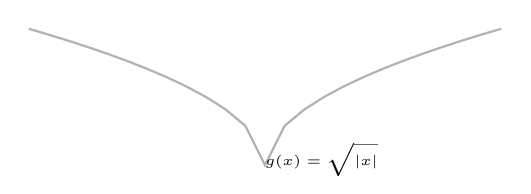
\begin{tikzpicture}[scale=1,draw opacity = 0.6]
		% abscisa y ordenada
		\tkzInit[xmax= 3,xmin=-3,ymax=3,ymin=0]
		\tiny\tkzLabelXY[opacity=0.6,step=1, orig=false]
		% etiqueta x, f(x)
		\tkzDrawX[opacity=0.6,label=x,right=0.3]
		\tkzDrawY[opacity=0.6,label=f(x),below = -0.6]
		%dominio y función
		\draw [domain=-3:3,thick,gray] plot(\x,{abs(\x)^(1/2)});
		\tkzText[opacity=0.6,above](1,1.7){\tiny $g(x)=\sqrt{|x|}$}
	    \end{tikzpicture}
	\end{center}
	\vspace{.5cm}

    %--------------------18.
    \item $g(x) = \sqrt{-x}$\\\\
	Respuesta.-\; El dominio de la función se cumple para los números reales negativos.   
	\begin{center}
	    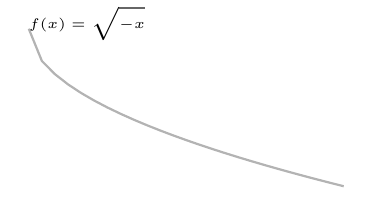
\begin{tikzpicture}[scale=1,draw opacity = 0.6]
		% abscisa y ordenada
		\tkzInit[xmax= 4,xmin=-1,ymax=1,ymin=-2]
		\tiny\tkzLabelXY[opacity=0.6,step=1, orig=false]
		% etiqueta x, f(x)
		\tkzDrawX[opacity=0.6,label=x,right=0.3]
		\tkzDrawY[opacity=0.6,label=f(x),below = -0.6]
		%dominio y función
		\draw [domain=0:4,thick,gray] plot(\x,{-\x^(1/2)});
		\tkzText[opacity=0.6,above](2,-1){\tiny $f(x)=\sqrt{-x}$}
	    \end{tikzpicture}
	\end{center}
	\vspace{.5cm}

    %--------------------19.
    \item $F(t)=t/|t|$\\\\
	Respuesta.-\; El dominio viene dado para todo número real menos el $0$. 
	\begin{center}
	    \begin{tikzpicture}[scale=1,draw opacity = 0.6]
		% abscisa y ordenada
		\tkzInit[xmax= 3,xmin=-3,ymax=2,ymin=-2]
		\tiny\tkzLabelXY[opacity=0.6,step=1, orig=false]
		% etiqueta x, f(x)
		\tkzDrawX[opacity=0.6,label=x,right=0.3]
		\tkzDrawY[opacity=0.6,label=f(x),below = -0.6]
		%dominio y función
		\draw [domain=.1:3,thick,gray] plot(\x,{\x/abs(\x)});
		\draw [domain=-3:-.1,thick,gray] plot(\x,{\x/abs(\x)});
		\tkzText[opacity=0.6,above](1,1){\tiny $F(t)=t/|t|$}
	    \end{tikzpicture}
	\end{center}
	\vspace{.5cm}

    %--------------------20.
    \item $G(t)=1/|t|$\\\\
	Respuesta.-\; El dominio se cumple para todo número real menos el $0$.
	\begin{center}
	    \begin{tikzpicture}[scale=1,draw opacity = 0.6]
		% abscisa y ordenada
		\tkzInit[xmax= 3,xmin=-3,ymax=5,ymin=0]
		\tiny\tkzLabelXY[opacity=0.6,step=1, orig=false]
		% etiqueta x, f(x)
		\tkzDrawX[opacity=0.6,label=x,right=0.3]
		\tkzDrawY[opacity=0.6,label=f(x),below = -0.6]
		%dominio y función
		\draw [domain=.2:3,thick,gray] plot(\x,{1/abs(\x)});
		\draw [domain=-3:-.2,thick,gray] plot(\x,{1/abs(\x)});
		\tkzText[opacity=0.6,above](2,2){\tiny $G(t)=1/|t|$}
	    \end{tikzpicture}
	\end{center}
	\vspace{.5cm}

    %--------------------21
    \item Determine el dominio de $y=\dfrac{x+3}{4-\sqrt{x^2-9}}$\\\\
	Respuesta.-\; Si $y=f(x)$ entonces el dominio esta dado por $D_f=\lbrace x / x\geq 3 \land x \neq 4 \rbrace$ \\\\

    %--------------------22.
    \item Determine el rango de $y=2+\dfrac{x^2}{x^2+4}$.\\\\
	Respuesta.-\; Si $y=f(x)$ entonces el rango viene dado para todo $y=f(x)$ tal que $y\geq 2$\\\\

    %--------------------23.
    \item Grafique las siguientes ecuaciones y explique por qué no son gráficas de funciones de $x$.\\\\
    
    \begin{enumerate}[\bfseries a.]
	
	%----------a.
	\item $|y|=x$\\\\
	    Respuesta.-\; No es una función de $x$ ya que $ \sqrt{y^2}=x \Longrightarrow y^2=x^2 \Longrightarrow \pm y = \pm x$\\\\

	%----------b.
	\item $y^2 = x^2$\\\\
	    Respuesta.-\; Por el anterior problema $23a.$\\\\
	
    \end{enumerate}

    %--------------------24.
    \item Grafique las siguientes ecuaciones y explique por qué no son gráficas de funciones de $x$\\\\

    \begin{enumerate}[\bfseries a.]

	%----------a.
	\item $|x|+|y|=1$\\\\
	    Respuesta.-\; Ya que $|y|=1 - |x| \Longrightarrow \sqrt{y^2} = 1 - |x| \Longrightarrow y^2 = (1-|x|)^2 \Longrightarrow \pm y= |1-|x||$\\\\

	%----------b.
	\item $|x+y|=1$\\\\
	Respuesta.-\;  Ya que $\sqrt{(x+y)^2}=1 \Longrightarrow (x+y)^2 = 1 \Longrightarrow x^2 + 2xy + y^2 = 1 \Longrightarrow y^2 = 1 - 2xy - x^2 \Longrightarrow \pm y = \sqrt{1-2xy-x^2}$\\\\
    \end{enumerate}

    Funciones definidas por partes\\\\
    En los ejercicios 25 a 28, grafique las funciones:\\\\

    %--------------------25.
    \item $f(x) = \left\{ \begin{array}{cc}
		    x,&0\leq x \leq 1\\
		    \\ 2-x,&1<x\leq 2 \\
		    \end{array} \right.$
	\begin{center}
	    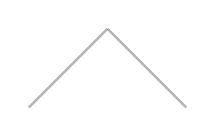
\begin{tikzpicture}[scale=1,draw opacity = 0.6]
		% abscisa y ordenada
		\tkzInit[xmax= 3,xmin=-1,ymax=2,ymin=0]
		\tiny\tkzLabelXY[opacity=0.6,step=1, orig=false]
		% etiqueta x, f(x)
		\tkzDrawX[opacity=0.6,label=x,right=0.3]
		\tkzDrawY[opacity=0.6,label=f(x),below = -0.6]
		%dominio y función
		\draw [domain=0:1,thick,gray] plot(\x,{\x});
		\draw [domain=1:2,thick,gray] plot(\x,{2-\x});
	    \end{tikzpicture}
	\end{center}
	\vspace{.5cm}
    
    %--------------------26.
    \item $g(x) = \left\{ \begin{array}{cc}
		    1-x,&0\leq x \leq 1\\
		    \\ 2-x,&1<x\leq 2 \\
		    \end{array} \right.$
	\begin{center}
	    
\begin{tikzpicture}[scale=1,draw opacity = 0.6]
		% abscisa y ordenada
		\tkzInit[xmax= 3,xmin=-1,ymax=2,ymin=0]
		\tiny\tkzLabelXY[opacity=0.6,step=1, orig=false]
		% etiqueta x, f(x)
		\tkzDrawX[opacity=0.6,label=x,right=0.3]
		\tkzDrawY[opacity=0.6,label=f(x),below = -0.6]
		%dominio y función
		\draw [domain=0:1,thick,gray] plot(\x,{1-\x});
		\draw [domain=1:2,thick,gray] plot(\x,{2-\x});
	    \end{tikzpicture}
	\end{center}
	\vspace{.5cm}
    
    %--------------------27.
    \item $F(x) = \left\{ \begin{array}{cc}
		    4-x^2,&\leq 1 \\
		    \\ x^2 + 2x,& x>1 \\
		    \end{array} \right.$
	\begin{center}
	    \begin{tikzpicture}[scale=1,draw opacity = 0.6]
		% abscisa y ordenada
		\tkzInit[xmax= 3,xmin=-3,ymax=8,ymin=0]
		\tiny\tkzLabelXY[opacity=0.6,step=1, orig=false]
		% etiqueta x, f(x)
		\tkzDrawX[opacity=0.6,label=x,right=0.3]
		\tkzDrawY[opacity=0.6,label=f(x),below = -0.6]
		%dominio y función
		\draw [domain=-2:1,thick,gray] plot(\x,{4-\x*\x});
		\draw [domain=1:2,thick,gray] plot(\x,{\x*\x + 2*\x});
	    \end{tikzpicture}
	\end{center}
	\vspace{.5cm}

    %--------------------28.
    \item $G(x) = \left\{ \begin{array}{cc}
		    1/x,&x<0\\
		    \\ x, & 0\leq x \\
		    \end{array} \right.$
	\begin{center}
	    \begin{tikzpicture}[scale=1,draw opacity = 0.6]
		% abscisa y ordenada
		\tkzInit[xmax= 3,xmin=-4,ymax=2,ymin=-8]
		\tiny\tkzLabelXY[opacity=0.6,step=1, orig=false]
		% etiqueta x, f(x)
		\tkzDrawX[opacity=0.6,label=x,right=0.3]
		\tkzDrawY[opacity=0.6,label=f(x),below = -0.6]
		%dominio y función
		\draw [domain=-3:0,thick,gray] plot(\x,{1*\x^(-1)});
		\draw [domain=0:2,thick,gray] plot(\x,{\x});
	    \end{tikzpicture}
	\end{center}
	\vspace{.5cm}

    Determine una fórmula para cada función graficada en los ejercicios $29$ a $32$\\\\

    %--------------------29
    \item 
    \begin{enumerate}[\bfseries a.]
	
	%----------a.
	\item  Sea $f(x)=ax+b$ entonces $0=b$ y $1=a+b$ luego $a=1$ por lo tanto $f(x)=x$. Por otro lado $1=a+b$ y $0=2a+2 \Longrightarrow a=-1$ de donde se tiene $f(x^{'})=-x+2$ así nos queda la función:
	$$f(x) = \left\{\begin{array}{r c l}
		x&si&0\leq x \leq 1\\
		\\ x+2&si&1\leq x \leq 2 \\
	    \end{array}\right.$$\\\\

	%----------b.
	\item Está definida por $$f(x)=\left\{\begin{array}{rcl} 
				    2&si&0\leq x < 1 \; y \; 2 \leq x < 3\\
				    \\  0&si& 1\leq x < 2 \; y \; 3\leq x \leq 4\\
				    \end{array}\right.$$\\\\

    \end{enumerate}

    %--------------------30.
    \item 
    \begin{enumerate}[\bfseries a.]

	%----------a.
	\item Similar al ejercicio anterior se tiene que la formula 
	$$f(x)= \left\{ \begin{array}{rcl}
		x+2&si& 0 \leq x \leq 2 \\
		\\ 1/2x+5/7&si& 0\leq x \leq 2 \\ \end{array}\right.$$\\\\

	%----------b.
	\item Se tiene 
	$$f(x)=\left\{\begin{array}{rcl} 
		-3x - 3&si&-1\leq x \leq 0\\
		\\-2x + 3&si&\\ \end{array} \right.$$\\\\

    \end{enumerate}

    %--------------------31.
    \item 
    \begin{enumerate}[\bfseries a.]

	%----------a.
	\item  
	$$f(x)= \left\{ \begin{array}{rcl}
		x+2&si& -1 \leq x < 0 \\
		\\ 1&si& 0 < x \leq 1 \\ 
		\\ -2x + 2&si&1 \leq x \leq 3\\
		\end{array}\right.$$\\\\
	
	%----------b.
	\item Sea $(a,b)$ y $(c,d)$ por lo tanto por capitulo $4$ de spivak $f(x)=\dfrac{d-b}{c-a}(x-a)+b$ entonces $(-2,-1)$ y $(0,0)$ así $f(x)=\dfrac{0-1}{0+2}(x+2) + 0 \quad \Longrightarrow \quad f(x) = -\dfrac{1}{2}x - 2$ \\\\
	Luego $f(x)=-2x+2$ y finalmente $f(x)=-1$ de donde,
	$$f(x)= \left\{ \begin{array}{rcl}
		- \dfrac{1}{2}x -2&si& -2 \leq x \leq 0 \\
		\\ 2x+2&si& 0 < x \leq 1 \\ 
		\\ -1&si&1 < x \leq 3\\
		\end{array}\right.$$\\\\
    \end{enumerate}

    %--------------------32.
    \item 
    \begin{enumerate}[\bfseries a.]

	%----------a.
	\item 
	$$f(x)= \left\{ \begin{array}{rcl}
		0&si& 0 \leq x \leq \dfrac{T}{2} \\\\
		\\ \dfrac{2x}{T} - 1&si& \dfrac{T}{2}< x \leq T \\\\ 
		\end{array}\right.$$\\\\

	%----------b.
	\item  
	$$f(x)= \left\{ \begin{array}{rcl}
		A&si& \dfrac{T}{2} \leq x < T \quad y \quad T \leq x < \dfrac{3T}{2}\\\\
		\\ -A&si&\dfrac{T}{2} \leq x < T \quad y \quad \dfrac{3T}{2} \leq x \leq 2T \\\\
		\end{array}\right.$$\\\\

    \end{enumerate}

Las funciones mayor entero y menor entero.\\\\

    %--------------------33.
    \item Para qué valores de $x$ es 
    \begin{enumerate}[\bfseries a.]
	\item $[x]=0$\\\\
	    respuesta.-\; Para $0\leq x < 1$\\\\
	\item $[x] =0$\\\\
	    Respuesta.-\; Para $-1 < x \leq 0$\\\\
    \end{enumerate}

    %--------------------34.
    \item ¿Cuáles valores $x$ de números reales satisfacen la ecuación $[x] = [x]$?\\\\
	Respuesta.-\; Sólo el $0$.\\\\

    %--------------------35.
    \item ¿Es cierto que $[-x] = -[x]$ para todo número real $x$? Justifique su respuesta.\\\\
	Respuesta.-\; Es cierto siempre y cuando sea $x$ un entero. Ya que si $x\in \mathbb{Z}$ entonces $x=n$ para algunos $n\in \mathbb{Z}$, por lo tanto $[x]=n$ y $-x=-n \Longrightarrow [-x] = n \Longrightarrow [-x] = -[x]$. Por otro lado sea $x \notin \mathbb{Z}$ y $[x]=n$ entonces  $n\leq x < n+1 \Longrightarrow -n-1<-x<-n \Longrightarrow [-x] = -n-1 = -[x] - 1$\\\\

    %--------------------36.
	\item Grafique la función 
		$$f(x) = \left\{\begin{array}{cl}
			[x],&x\leq 0\\
			 x,&x<0\\
			\end{array}\right.$$ 
	    ¿Por qué $f(x)$ se donomina parte entera de $x$?\\\\
	    Respuesta.-\; Se denomia porque hace corresponder el número inmediato anterior.\\\\

    Funciones crecientes y funciones decrecientes.\\\\
    Grafique las funciones en los ejercicios 37 a 46. Si tiene simetrías, ¿Qué tipo de simetría tienen? Especifique los intervalos en os que la función es creciente y los intervalos donde la función es decreciente.\\\\ 

    %--------------------37
    \item $y=-x^3$
	\begin{center}
	    \begin{tikzpicture}[scale=1,draw opacity = 0.6]
		% abscisa y ordenada
		\tkzInit[xmax= 2,xmin=-2,ymax=2,ymin=-2.2]
		\tiny\tkzLabelXY[opacity=0.6,step=1, orig=false]
		% etiqueta x, f(x)
		\tkzDrawX[opacity=0.6,label=x,right=0.3]
		\tkzDrawY[opacity=0.6,label=f(x),below = -0.6]
		%dominio y función
		\draw [domain=-1.3:1.3,thick,gray] plot(\x,{-\x^3});
	    \end{tikzpicture}
	\end{center}
	\vspace{.5cm}
	Respuesta.-\; Tiene simetría impar y el intervalo donde decrece esta dado por $(-\infty,\infty)$\\\\

    %--------------------38.
    \item $y=-\dfrac{1}{x^2}$\\\\
	Respuesta.-\; Tiene simetría par y esta dado por lo el intervalo decreciente de $-\infty<x<0$ y por el intervalo creciente $0<x<\infty$

    %--------------------39.
    \item $y=-\dfrac{1}{x}$\\\\
	Respuesta.-\; Tiene simetría impar y viene dado por los intervalos crecientes $-\infty < x < 0$  y $0<x<\infty$\\\\

    %--------------------40.
    \item $y=\dfrac{1}{|x|}$\\\\
	Respuesta.-\; Tiene simetría par y viene dado por el intervalo creciente $-\infty<x<0$ y el intervalo decreciente $0<x<\infty$\\\\

    %--------------------41.
    \item $y=\sqrt{|x|}$\\\\
	\begin{center}
	    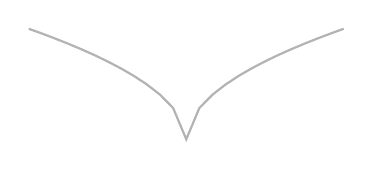
\begin{tikzpicture}[scale=1,draw opacity = 0.6]
		% abscisa y ordenada
		\tkzInit[xmax= 2,xmin=-2,ymax=2,ymin=0]
		\tiny\tkzLabelXY[opacity=0.6,step=1, orig=false]
		% etiqueta x, f(x)
		\tkzDrawX[opacity=0.6,label=x,right=0.3]
		\tkzDrawY[opacity=0.6,label=f(x),below = -0.6]
		%dominio y función
		\draw [domain=-2:2,thick,gray] plot(\x,{sqrt(abs(\x))});
	    \end{tikzpicture}
	\end{center}
	\vspace{.5cm}
	Respuesta.-\; Tiene simetría par y esta dado por el intervalo  decreciente  $-\infty < x \leq 0$ y el intervalo creciente $0\leq x < \infty$\\\\

    %--------------------42.
    \item $y=\sqrt{-x}$\\\\
	\begin{center}
	    \begin{tikzpicture}[scale=1,draw opacity = 0.6]
		% abscisa y ordenada
		\tkzInit[xmax= 2,xmin=-2,ymax=2,ymin=0]
		\tiny\tkzLabelXY[opacity=0.6,step=1, orig=false]
		% etiqueta x, f(x)
		\tkzDrawX[opacity=0.6,label=x,right=0.3]
		\tkzDrawY[opacity=0.6,label=f(x),below = -0.6]
		%dominio y función
		\draw [domain=-2:0,thick,gray] plot(\x,{sqrt(-\x)});
	    \end{tikzpicture}
	\end{center}
	\vspace{.5cm}
	Respuesta.- No es ni par ni impar y viene dado por el intervalo decreciente $-\infty < x \leq 0$\\\\

    %-------------------43.
    \item $y=x^3/8$\\\\
	\begin{center}
	    \begin{tikzpicture}[scale=1,draw opacity = 0.6]
		% abscisa y ordenada
		\tkzInit[xmax= 3,xmin=-3,ymax=2,ymin=-2]
		\tiny\tkzLabelXY[opacity=0.6,step=1, orig=false]
		% etiqueta x, f(x)
		\tkzDrawX[opacity=0.6,label=x,right=0.3]
		\tkzDrawY[opacity=0.6,label=f(x),below = -0.6]
		%dominio y función
		\draw [domain=-2.5:2.5,thick,gray] plot(\x,{\x^3/8});
	    \end{tikzpicture}
	\end{center}
	\vspace{.5cm}
	Respuesta.-\; Tiene simetría impar y viene dado por el intervalo creciente $-\infty < x < \infty$\\\\

    %---------------------44.
    \item $y=-4\sqrt{x}$\\\\
	\begin{center}
	    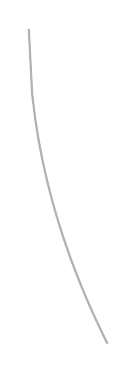
\begin{tikzpicture}[scale=1,draw opacity = 0.6]
		% abscisa y ordenada
		\tkzInit[xmax= 2,xmin=-1,ymax=1,ymin=-4]
		\tiny\tkzLabelXY[opacity=0.6,step=1, orig=false]
		% etiqueta x, f(x)
		\tkzDrawX[opacity=0.6,label=x,right=0.3]
		\tkzDrawY[opacity=0.6,label=f(x),below = -0.6]
		%dominio y función
		\draw [domain=0:1,thick,gray] plot(\x,{-4*sqrt(\x)});
	    \end{tikzpicture}
	\end{center}
	\vspace{.5cm}
	Respuesta.-\; No es ni par ni impar y viene dado por el intervalo $0\leq x < \infty$\\\\

    %--------------------45.
    \item $y=-x^{3/2}$\\\\
	\begin{center}
	    \begin{tikzpicture}[scale=1,draw opacity = 0.6]
		% abscisa y ordenada
		\tkzInit[xmax= 2,xmin=-1,ymax=1,ymin=-1]
		\tiny\tkzLabelXY[opacity=0.6,step=1, orig=false]
		% etiqueta x, f(x)
		\tkzDrawX[opacity=0.6,label=x,right=0.3]
		\tkzDrawY[opacity=0.6,label=f(x),below = -0.6]
		%dominio y función
		\draw [domain=-1:1,thick,gray] plot(\x,{-(\x^(3/2))});
	    \end{tikzpicture}
	\end{center}
	\vspace{.5cm}
	Respuesta.-\; Tiene simetría impar y viene dado por el intervalo decreciente $-\infty < x < \infty$\\\\

    %---------------------46.
    \item $y=(-x)^{2/3}$\\\\
	\begin{center}
	    \begin{tikzpicture}[scale=1,draw opacity = 0.6]
		% abscisa y ordenada
		\tkzInit[xmax= 2,xmin=-1,ymax=1,ymin=-1]
		\tiny\tkzLabelXY[opacity=0.6,step=1, orig=false]
		% etiqueta x, f(x)
		\tkzDrawX[opacity=0.6,label=x,right=0.3]
		\tkzDrawY[opacity=0.6,label=f(x),below = -0.6]
		%dominio y función
		\draw [domain=-1:1,thick,gray] plot(\x,{\x^(2/3)});
	    \end{tikzpicture}
	\end{center}
	\vspace{.5cm}
	Respuesta.-\; La simetría es impar y viene dado por el intervalo creciente $-\infty < x < \infty$\\\\

    Funciones pares y funciones impares \\\\
    En los ejercicios $47$ a $58$, indique si la función es par, impar o de ninguno de estos tipos. Justifique su respuesta.\\\\

    %--------------------47.
    \item $f(x)=3$\\\\
	Respuesta.-\; Sea $f(-x)=3=f(x)$ entonces decimos que la función es par.\\\\

    %--------------------48.
    \item $f(x)=x^{-5}$\\\\
	Respuesta.-\; Sea $f(-x)=(-x)^{-5} = -\left(x^{-5}\right)=-f(x)$, por lo tanto la función es impar.\\\\

    %--------------------49.
    \item $f(x)=x^2 + 1$\\\\
	Respuesta.-\; Sea $f(-x)=(-x)^2 + 1 = x^2 + 1 = f(x)$, de donde se tiene que la función es par.\\\\

    %--------------------50.
    \item $f(x)=x^2 + x$\\\\
	Respuesta.-\; Sea $f(-x)=(-x)^2 + (-x) = x^2 - x$ de donde la función no es par ni impar.\\\\

    %--------------------51.
    \item $g(x)=x^3  + x$\\\\
	Respuesta.-\; Sea $f(-x) = (-x)^3 + (-x) = -(x^3 + x) = -f(x)$ por lo tanto la función es impar.\\\\

    %--------------------52.
    \item $g(x)=x^4 + 3x^2 - 1$\\\\
	Respuesta.-\; Sea $g(-x) = (-x)^4 + 3(-x)^2 - 1 = g(x)$ por lo tanto la función es par.\\\\

    %--------------------53.
    \item $g(x)=\dfrac{1}{x^2-1}$\\\\
	Respuesta.-\; Sea $g(-x)=\dfrac{1}{(-x)^2 - 1} = g(x)$ por lo tanto la función es par.\\\\

    %--------------------54.
    \item $g(x)=\dfrac{x}{x^2 - 1}$\\\\
	Respuesta.-\; Sea $g(-x)=\dfrac{-x}{(-x)^2 - 1} = - \dfrac{x}{x^2 - 1} = -g(x)$ de donde la función es impar.\\\\

    %--------------------55.
    \item $h(t)=\dfrac{1}{t-1}$\\\\
	Respuesta.-\; Sea $h(-t)=\dfrac{1}{-t-1}$ entonces la función no es par ni impar.\\\\

    %--------------------56.
    \item $h(t)=|t^3|$\\\\
	Respuesta.-\; Sea $h(-t)=|(-t)^3| = |t^3| = h(t)$ por lo tanto la función es par.\\\\

    %--------------------57.
    \item $h(t)=2t+1$\\\\
	Respuesta.-\; Sea $h(-t) = 2(-t) + 1$ entonces la función no es ni par ni impar.\\\\

    %--------------------58.
    \item $h(t)=2|t|+1$\\\\
	Respuesta.-\; Sea $h(-t)=2|-t| + 1 = 2t + 1 = h(t)$ entonces la función es par.\\\\

    Teoría y ejemplos\\\\

    %--------------------59.
    \item La variable $s$ es proporcional a $t$, y $s=25$ cuando $t=75$. Determine $t$ cuando $s=60.$\\\\
	Respuesta.-\; Sea $\dfrac{s}{r}$ entonces $\dfrac{25}{75}=\dfrac{60}{x} \quad \Rightarrow \quad \dfrac{1}{3} = \dfrac{60}{x} \quad \Rightarrow \quad x=180$\\\\ 

    %--------------------60.
    \item Energía cinética. La energía cinética $K$ de una masa es proprocional al cuadrado de su velocidad $v$. Si $K=12,960$ joules, cuando $v=18$ m/s, ¿Cuál es el valor de $K$ cuando $v=10$ m/s?.\\\\
	Respuesta.-\; Similar al anterior ejercicio se tiene $\dfrac{K}{v^2} = \dfrac{12,960}{18^2} = \dfrac{K}{10^2}$ entonces $K=4000$.\\\\

    %--------------------61.
    \item Las variables $r$ y $s$ son inversamente proporcional, mientras que $r=6$ cuando $s=4$. Determine $s$ cuando $r=10$.\\\\
	Respuesta.-\; Tenemos que $6\cdot 4 = s \cdot 10$ entonces queda que $s = 2.4$.\\\\

    %--------------------62.
    \item Ley de Boyle. La ley de Boyle establece que el volumen $V$ de un gas, a temperatura constante, aumenta cuando la presión $P$ disminuye, de manera que $V$ y $P$ son inversamente proporcionales. Si $P = 14.7 lb/in^2$ cuando $V = 1000 in^3$, entonces ¿cuál es el valor de $V$ cuando $P = 23.4 lbs/in^2$?.\\\\
	Respuesta.-\; Sea $V\cdot P = V^{'} \cdot P^{'}$ entonces $14.7 \cdot 1000 = V \cdot 23.4$ y por lo tanto $V=628.2 in^3$.\\\\

    %--------------------63.
    \item Una caja sin tapa se construye a partir de una pieza rectangular de cartón, cuyas dimensiones son $14$ por $22$ pulgadas (in). A la pieza de cartón se le cortan cuadrados de lado $x$ en cada esquina y luego se doblan hacia arriba los lados, como en la figura. Exprese el volumen $V$ de la caja como una función de $x$.\\\\
	Respuesta.-\; El volumen es dado por $V=L\cdot a\cdot h$ luego $h=x,\qquad a=14-2x, \qquad L=22-2x$ por lo tanto $$V(x)=(22-2x)(14-2x)\cdot x \quad \Longrightarrow \quad V(x)=4x^3 - 72x^2 + 308x$$\\\\

    %--------------------64.
    \item La siguiente figura muestra un rectángulo inscrito en un triángulo rectángulo isósceles, cuya hipotenusa tiene una longitud de dos unidades.
    \begin{enumerate}[\bfseries a.]
	
	%----------a.
	\item Exprese la coordenada de $P$ en términos de $x$. (Podría iniciar escribiendo una ecuación para la recta $AB$).\\\\
	    Respuesta.-\; Sea $y=mx+b$ luego en el punto $B$, se tiene la intersección de ambas rectas que forman un ángulo de $90^{°}$, así que, el ángulo que tiene que tener el punto $A$ es de $45^{°}$ o bien $m=-1$ por lo tanto $y=-x+b$ o bien m=-1 ya que la recta va hacia abajo.\\\\

	%----------b.
	\item Exprese el área del rectángulo en términos de $x$.\\\\
	    Respuesta.-\; El área de un rectángulo es $b\cdot a$ de donde $area = 2x \cdot y = 2x(b-x)$.\\\\

    \end{enumerate}

    En los ejercicios 65 y 66 relacione cada ecuación con su gráfica. No utilice un dispositivo para graficar y dé razones que justifiquen su respuesta.\\\\

    %--------------------65.
    \item  
    \begin{enumerate}[\bfseries a.]
	
	%----------a.
	\item $y=x^4 \quad \Rightarrow \quad h$\\\\

	%----------b.
	\item $y=x^7 \quad  \Rightarrow \quad f$\\\\

	%----------c.
	\item $y=x^10 \quad \Rightarrow \quad g$\\\\

    \end{enumerate}

    %--------------------66.
    \item
    \begin{enumerate}[\bfseries a.]
	
	%----------a.
	\item $y=5x \quad \Rightarrow \quad f$.\\\\

	%----------b.
	\item $y=5x \quad \Rightarrow \quad f$.\\\\

	%----------c.
	\item $y=x^5 \quad \Rightarrow \quad h$.\\\\

    \end{enumerate}

    %--------------------67.
    \item 
    \begin{enumerate}[\bfseries a.]

	%----------a.
	\item Grafique juntas las funciones $f(x)=x/2$ y $g(x)=1+(4/x)$ para identificar los valores de $x$ que satisfacen $$\dfrac{x}{2} > 1 + \dfrac{4}{x}$$\\
	\begin{center}
	    \begin{tikzpicture}[scale=1,draw opacity = 0.6]
		% abscisa y ordenada
		\tkzInit[xmax= 6,xmin=-4.5,ymax=3,ymin=-2]
		\tiny\tkzLabelXY[opacity=0.6,step=1, orig=false]
		% etiqueta x, f(x)
		\tkzDrawX[opacity=0.6,label=x,right=0.3]
		\tkzDrawY[opacity=0.6,label=f(x),below = -0.6]
		%dominio y función
		\draw [domain=-3:6,thick,gray] plot(\x,{\x/2});
		\draw [domain=2:6,thick,gray] plot(\x,{1+(4/\x)});
		\draw [domain=-4:-1.5,thick,gray] plot(\x,{1+(4/\x)});
	    \end{tikzpicture}
	\end{center}
	\vspace{.5cm}

	%----------b.
	\item Confirme algebraicamente los hallazgos del inciso $a)$\\\\
	    Respuesta.-\; Resolviendo la ecuación nos queda $x^2-2x-8>0$ donde se cumple para $x>4$ ó $x<-2$\\\\

    \end{enumerate}

    %--------------------68.
    \item 
    \begin{enumerate}[\bfseries a.]
	
	%----------a.
	\item Grafique juntas las funciones $f(x) = 3/(x-1)$ y $g(x)=2/(x+1)$ para identificar los valores de $x$ que satisfacen $$\dfrac{3}{x-1}<\dfrac{2}{x+1}$$\\
	\begin{center}
	    
\begin{tikzpicture}[scale=1,draw opacity = 0.6]
		% abscisa y ordenada
		\tkzInit[xmax= 1,xmin=-12,ymax=1,ymin=-2]
		\tiny\tkzLabelXY[opacity=0.6,step=1, orig=false]
		% etiqueta x, f(x)
		\tkzDrawX[opacity=0.6,label=x,right=0.3]
		\tkzDrawY[opacity=0.6,label=f(x),below = -0.6]
		%dominio y función
		\draw [domain=-11:-3,thick,gray] plot(\x,{3/(\x-1)});
		\draw [domain=-11:-3,thick,gray] plot(\x,{2/(\x+1)});
	    \end{tikzpicture}
	\end{center}
	\vspace{.5cm}

	%----------b.
	\item Confirme algebraicamente los hallazgos del inicio $a)$.\\\\
	    Respuesta.-\; Sea $\dfrac{3}{x-1}<\dfrac{2}{x+1} \quad \Rightarrow \quad x<-5$\\\\

    \end{enumerate}

    %-------------------69.
    \item Para que una curva sea simétrica con respecto al eje $x$, el punto $(x, y)$ debe estar en la curva si y sólo si el punto $(x, -y)$ está en la curva. Explique por qué una curva que es simétrica con respecto al eje $x$ no es la gráfica de una función a menos que la función sea $y = 0$.\\\\
	Respuesta.-\; Esto se debe a que contradice a la definición de función. Es decir, a cada elemento $x$ se asigna un solo o único elemento $f(x)$. Si $y=0$ entonces $(x,y)=(x,-y)$ y por lo tanto se cumple la definición de función\\\\

    %--------------------70.
    \item Trescientos libros se venden en $\$ 40$ cada uno, lo que da por resultado un ingreso de $300\cdot \$ 40 $ = $\$12,000$. Por cada aumento de $\$ 5$ en el precio, se venden $25$ libros menos. Exprese el ingreso $R$ como una función del número $x$ de incrementos de $\$5$.\\\\
	Respuesta.-\; Veamos algunos ejemplos particulares:
	\begin{center}
	    \begin{tabular}{rcl}
		$300\cdot 40$&$=$&$12000$\\
		$(300 - 25)(40 + 5)$&$=$&$12375$\\
		$(300 - 50)(40 + 10)$&$=$&$12500$\\
		$(300 - 75)(40 + 15)$&$=$&$12375$\\
		$(300 - 100)(40 + 20)$&$=$&$12000$\\
	    \end{tabular}
	\end{center}
	Por lo tanto $R(x)=(300-5x)(40+x)=-125x^2 + 500x + 12000$\\\\

    %--------------------71.
    \item Se va a construir un corral con la forma de un triángulo rectángulo isósceles con catetos de longitud de $x$ pies (ft) e hipotenusa de longitud $h$ ft. Si los costos de la cerca son de $\$ 5 / ft$ para los catetos y $\$ lO/ft$ para la hipotenusa, escriba el costo total $C$ de la construcción como una función de $h$.\\\\
	Respuesta.-\; Sea $c^2+c^2=h^2 \quad \Rightarrow \quad h=c \sqrt{2} \quad \Rightarrow \quad c=h \sqrt{2}$, luego $C=2\cdot c \cdot 5 + h \cdot 10$ por lo tanto $C=10\cdot h \dfrac{1}{\sqrt{2}} + 1$\\\\

    %--------------------72.
    \item Costos industriales: Una central eléctrica se encuentra cerca de un río, donde éste tiene un ancho de 800 ft. Tender un cable de la planta a un lugar en la ciudad, 2 millas (mi) río abajo en el lado opuesto, tiene un costo de $180 por ft que cruce el río y $100 por ft en tierra a lo largo de la orilla del río.
    \begin{enumerate}[\bfseries a.]

	%----------a.
	\item Suponga que el cable va de la planta al punto $Q$, en el lado opuesto, lugar que se encuentra a $x$ ft del punto $P$, directamente opuesto a la planta. Escriba una función $C(x)$ que indique el costo de tender el cable en términos de la distancia $x$.\\\\
	    Respuesta.-\; Por el teorema de Pitágoras podemos establecer la función $C(x)$ como sigue: $$C(x)=\sqrt{x^2 + 800^2} \cdot 180 + (10560-x)\cdot 100$$

	%----------b.
	\item Genere una tabla de valores para determinar si la ubicación más barata para el punto $Q$ es menor a $2000$ ft o mayor a $2000$ ft del punto $P$.\\\\
	    Respuesta.-\;
	    \begin{center}
		\begin{tabular}{rclcl}
		    $C(x)$&$=$&$\sqrt{1900^2+800^2} + (10560-1900)\cdot 100$&$=$&$1270599.7$\\
		    $C(x)$&$=$&$\sqrt{2100^2+800^2} + (10560-2100)\cdot 100$&$=$&$1217079.5$\\\\
		\end{tabular}
	    \end{center}
	    Por lo tanto es mas barato ubicar el punto $Q$ a una distancia mayor a $2000$ ft.\\\\

    \end{enumerate}

\end{enumerate}

\section{Ejercicios}

\begin{enumerate}[\Large \bfseries 1.]

%--------------------1.
\item
\end{enumerate}
